\documentclass[10pt,conference,compsocconf]{IEEEtran}

\usepackage{hyperref}
\usepackage{graphicx}	% For figure environment


\begin{document}
\title{Higgs Boson: a Machine Learning Challenge}

\author{
  Timothée Duran, Marijn van der Meer, Bradley Mathez
}

\maketitle

\begin{abstract}

 In this paper, we present our approach to the Higgs boson machine learning challenge. Different simple machine learning models were evaluated on the data set resulting from the Higgs boson experiment. Our objective was to find the model that would best predict the Higgs boson decay signatures from background noise by binary classification. For this, one model was chosen, regularized logistic regression, and was optimized to obtain the best accuracy and the smallest loss.  
\end{abstract}

\section{Introduction}\label{sec: introduction}
The Higgs boson, generated by quantum excitation of the Higgs field, is an elementary particle discovered at CERN in 2013. Rarely, a collision between protons generates a Higgs boson that then decays rapidly. The decay does, however, leave a signature that can be measured. In this project, the decay signatures, which come from the ATLAS~\cite{Aad_2012} and CMS  ~\cite{Chatrchyan_2012} that led to the discovery of this particle, were introduced into machine learning models in order to find an accurate binary classifier. The objective was to develop a model that would allow the identification of the Higgs boson signatures from background noise.
\section{Models and Methods}\label{sec: models_methods}
  \subsection{Pre-processing}\label{subsec:pre-proc}
  \subsubsection{Data}\label{subsubsec:data}
  The data provided was a training set of 250'000 events of 30 features and a test set of around 568'238 events. Features types varied from floating points to integer values and labels provided were -1 for background, and 1 for boson. Those were changed to 1 for boson and 0 for background for computational reasons with logistic regression. 
\subsubsection{Invalid values}\label{subsubsec:invalid_values}
Starting by plotting histograms for each of the 30 features of the raw data, we noticed that 10 out of 30 of the features had samples with invalid $-999$ values.   This can be
seen for one example feature in Fig.\ref{fig:example_pre_procs}. Because invalid values were present in significant numbers (around 100'000 for some features), removing those samples would have reduced our data almost by half and probably substantially impacted our training performance. Thus, to process these invalid samples, we replaced them with the median of the corresponding features without the invalid samples. We chose the median compared to the average as it is more robust to outliers. We mirrored the same process with the test set.
\subsubsection{Outliers}\label{subsubsec:outliers}
  Following the invalid values replacement, we searched for outliers in the data by applying the interquartile range rule, i.e. considering as outliers all samples $\leq Q_1-1.5IQR$ or $\geq Q_3+1.5IQR$ where $Q_1$ is the 25\% percentile and $Q_3$ the 75\%. In a first attempt, we lowered $Q1$ to $10\%$ and changed to the median all values $\leq 10\%(data)-1.5IQR$ or $\geq Q_3+1.5IQR$. Later, we noticed that our performance was greatest when removing only samples that were above  $85\%(data)+1.5IQR$. This reduced the training dataset from 250000 to 215311 samples and improved the accuracy of our model from 77\% to 81\%. The fact  that only removing "high tail" values improved our model might have been due to the fact that most features were positively skewed.  
  \subsection{Feature engineering}\label{subsec: feature_generation}
    After invalid values and outliers were processed, we engineered our features by applying a polynomial kernel to our data. This added a bias column and a polynomial expansion of the form $\phi:[X]\rightarrow [1, X, X^2,...,X^k]$ where $X\in \mathbb{R}^{N\times30}$. The data was then further standardised using Z-score standardisation: $Z = \frac{X - \mu}{\sigma}$ where $\mu$ is the mean and $\sigma$ the standard deviation of our expanded data. The same process was applied to the test set, the exception being that the test set was standardized according to the mean and standard deviation of the training set and not the test. An example of final training feature distribution after pre-processing and feature engineering can be seen again Fig.\ref{fig:example_pre_procs}.
    
  \subsection{
  Model implementation
  }\label{subsec:model_impl}
  To fit our data, we implemented six different models: 
    \begin{itemize}
        \item Linear regression using normal equations, gradient descent and stochastic gradient descent 
        \item Ridge regression using normal equations
        \item Logistic regression using gradient descent 
    \end{itemize}
    We chose to implement logistic regression with gradient descent rather than stochastic gradient descent as we were required to take batch-size 1 and noticed that this created great oscillations. \newline
    These different models were evaluated based on their loss and accuracy on validation sets created from a $80\%/20\%$ training/validation 5-fold cross-validation. To create some kind of baseline, we evaluated all models over 100 epochs with the same learning rate of 0.01, regularisation parameter of 0.02 and polynomial expansion of degree 2. From this, we observed that (regularised) logistic regression performed much better than the others (c.f. Table~\ref{tab:basic_training}). Thus, rather than tuning all of the models in order to improve their scores, we chose to concentrate on regularised logistic regression as it seemed the most promising from the start. 
    
    \subsection{Hyper-parameter tuning}\label{subsubsec: parameter_tuning}
    To tune the hyper-parameters of our (regularised) logistic regression model, we performed a randomized grid search~\cite{jonasbenner2019} whose aim of a randomized grid search is to pick $k$ random combinations from a grid of possible. We chose this approach compared to a classical grid search in order to reduce the computational and time price. Randomized grid search was used with 50 random picks on learning rates from  $[0.03,0.8]$, regularization parameters from $[0.001,0.1]$, and degree of polynomial expansion from $[1,7]$. The performance (validation loss) of parameters was again evaluated using 5-fold cross-validation and the combination resulting in minimal loss was kept.
    
\section{Results}\label{sec: results}
Following hyper-parameter tuning and some fine-tuning done by hand, regularized logistic regression produced the highest average validation accuracy for the following parameters: 
\begin{itemize}
    \item Learning rate: 0.8
    \item Regularization: 0.02
    \item Number of epochs: 500
    \item Degree of polynomial feature expansion: 3
\end{itemize}
Like mentioned in~\ref{subsec:model_impl}, validation accuracy and loss were evaluated over 5-fold cross-validation and results can be found in Table~\ref{tab:result_log_reg} and Fig.\ref{fig:train_val_lr}. As can be seen in Fig.\ref{fig:train_val_lr}, both losses decrease rapidly in the first 100 epochs and then more slowly as they tend towards the optimum for these parameters. The best fold gave a validation loss of 0.4187 and accuracy of 81.12\%, which corresponded to 80.1\% accuracy and 68.7\% F1 score on AIcrowd. 
\begin{figure}
  \centering
  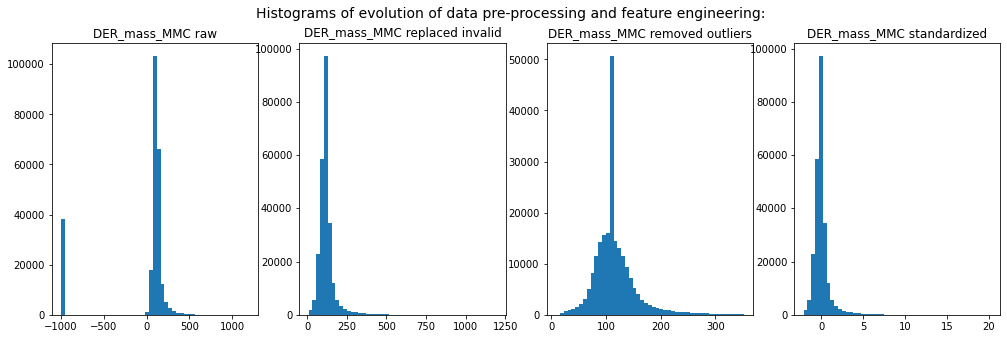
\includegraphics[width=\columnwidth]{report/example_pre_procs.png}
  \caption{Histogram of DER\_mass\_MMC samples. From left to right: raw data, data after replacing invalid values with median, removing outliers and standardizing}
  \vspace{-3mm}
  \label{fig:example_pre_procs}
\end{figure}

\begin{figure}
  \centering
  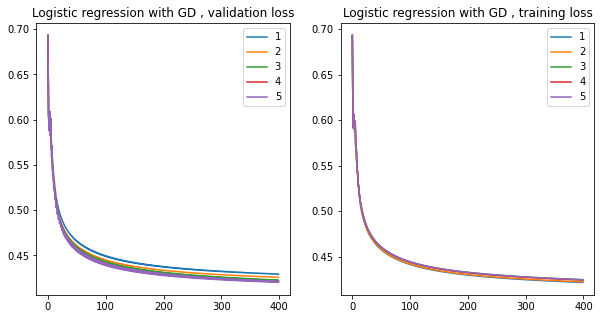
\includegraphics[width=\columnwidth]{report/train_val_loss.png}
  \caption{Validation and training loss evolution over 400 epochs, 5-folds and hyperparameters as mentioned in~\ref{sec: results}}.
  \vspace{-3mm}
  \label{fig:train_val_lr}
\end{figure}
\section{Discussion}\label{sec: discussion}
As can be seen in Fig.\ref{fig:train_val_lr}, the validation loss curve flattens out steadily after approximately 200 epochs, suggesting that no major performance improvements can be achieved by training for a longer time except for some 0.1\% changes. Interestingly, we noticed that changing the regularization parameter had little to no influence on the performance of our model. This might suggest that there is little overfitting happening with this choice of hyper-parameters. To further support this hypothesis, we notice that the training curve flattens out similarly to the validation curve and does not steadily decrease; which would suggest overfitting. \newline
In the future, to improve our results even further, we could do a more extensive grid search to try out more combinations of parameters and do a more thorough pre-processing of our raw data. Other outlier possibilities and ranges could be evaluated, and a better look at invalid values and how best to replace/remove them should be considered. Furthermore, as mentioned before, we noticed that some feature distribution were positively skewed. To improve training performance, we could therefore also try to apply a log transformation to those in order to try to render them more normal. 
\section{Conclusion}\label{sec: conclusion}
In conclusion, the best performance on the Higgs boson experiment data-set was attained with a model of regularized logistic regression with a high learning rate and little regularization. This was further enhanced by data cleaning and feature engineering, a process that could be further refined to achieve even better results.  



\begin{table}[]
  \centering
  \begin{tabular}[c]{|l||l|l|l|}
    \hline
    &Average loss&Average accuracy \\
    \hline
    Least squares GD & 0.18 & 50.16\% \\
    Least squares SGD & 0.29 & 50.90\%\\
    Least squares Normal & 0.15 & 42.68\%\\
    Ridge regression Normal & 0.15 & 42.68\%\\
    Logistic regression GD & 0.58 & 73.24\%\\
    Regularized logistic regression GD & 0.58 & 73.24\% \\
    \hline
  \end{tabular}
  \caption{Accuracy and loss on 20\% validation set for 100 epochs, learning rate of 0.01 and regularization of 0.02. }
  \label{tab:basic_training}
\end{table}

\begin{table}[htbp]
  \centering
  \begin{tabular}[c]{|l||l|l|l|}
    \hline
    &Final loss&Final accuracy \\
    \hline
    K = 1 & 0.4272 & 80.46 \% \\
    K = 2 &0.4238 & 80.56 \%\\
    K = 3 &0.4198 & 80.70 \%\\
    K = 4 &0.4188 & 81.12 \%\\
    K = 5 & 0.4193 & 81.01 \%\\
     \hline
    Average & 0.4265 & 80.78 \% \\
    \hline
  \end{tabular}
  \caption{Accuracy and loss on 20\% validation set for 400 epochs, learning rate of 0.8 and regularization of 0.02 for regularized logistic regression. }
  \label{tab:result_log_reg}
\end{table}


\bibliographystyle{IEEEtran}
\bibliography{literature}

\end{document}
